\documentclass[8pt,a4paper]{extarticle}
\usepackage[a4paper,margin=9mm,top=8mm,bottom=8mm]{geometry}
\usepackage[T1]{fontenc}
\usepackage{lmodern}
\usepackage{microtype}
\usepackage{booktabs,tabularx,array,multicol,amssymb}
\usepackage{xcolor}
\usepackage{tikz}
\usetikzlibrary{positioning,arrows.meta,fit}
\usepackage{enumitem}
\setlist{nosep,leftmargin=*}
\setlength{\parindent}{0pt}
\setlength{\parskip}{1.5pt}
\setlength{\columnsep}{4mm}
\setlength{\tabcolsep}{2.2pt}
\renewcommand{\arraystretch}{1.02}
\definecolor{edge}{HTML}{1F6F5C}
\definecolor{cloud}{HTML}{6B4C9A}
\definecolor{note}{HTML}{8A5A00}
\newcolumntype{L}[1]{>{\raggedright\arraybackslash}p{#1}}
\newcolumntype{Y}{>{\raggedright\arraybackslash}X}
\newcommand{\fn}[1]{{\fontsize{5.6}{6.4}\selectfont\ttfamily #1}}
\newcommand{\nm}{\textcolor{note}{\textit{not measured}}}
\newcommand{\hd}[1]{\textbf{\textcolor{edge}{#1}}}
\pagestyle{empty}

\begin{document}
{\centering
{\large\bfseries Offshore rig inspection \& repair fleet --- policy technical report}\\[1pt]
{\footnotesize Go2 quadruped + lift + UR3 arm (scrubber / sprayer / torque tool). Every number below is read from a
file in the repository (\texttt{runs\_sample/}, \texttt{policy/SCRUB.md}, \texttt{detection/RESULTS.md}, run summaries);
\emph{all results are simulation results} (Isaac Lab or CPU mocks) --- nothing has run on hardware yet.}\par}
\vspace{2pt}

\footnotesize
\noindent\begin{tabularx}{\textwidth}{@{}L{1.85cm}L{4.05cm}L{2.45cm}L{3.75cm}L{1.95cm}Y@{}}
\toprule
\textbf{Policy} & \textbf{Conditioned on (observation)} & \textbf{Action / output} & \textbf{How trained / designed} &
\textbf{Runs on $\cdot$ latency} & \textbf{Headline measured result} \\
\midrule
\textbf{1 Rust scrub PPO v2} \newline \fn{Rig-Scrub-}\newline\fn{Go2UR3Lift-v2} &
327-D: UR3 $q,\dot q$ (12); brush pos/vel in pipe frame (6); gap, $\sin\theta,\cos\theta$, axial (4); target$-$brush (3);
contact force $F$, setpoint $F^*$, pipe radius (3); $9{\times}9$ rust patch + $9{\times}9$ sprayed patch under brush (162);
$8{\times}16$ coarse rust map (128); nearest-rust vector + dist (3); rust left, unsprayed-contact flag (2); last action (4) &
4-D @30\,Hz: brush-target step in pipe frame ($\pm$1\,cm/axis) + $F^*{=}25{\pm}20$\,N; $F^*$ clipped at 38\,N outside the
net; DLS IK $\to$ UR3 joint targets &
rsl\_rl PPO, MLP 512-256-128 ELU, 24 steps/env. v1: 2048 envs$\times$150 it on GB10 ($\approx$9 min); v2 = 3-stage
fine-tune (150+200+150 it). Reward: $+50\,\Delta$removed, $+20$ success, contact band 10--40\,N, over-force
$1.0\frac{F-40}{10}+4\big(\frac{F-30}{10}\big)^2_{+}$, unsprayed, action-rate. DR: spring $k$ 1.5--4\,kN/m, abrasion
0.5--1.5, 1--4 patches, pipe yaw $\pm$10$^\circ$, new patch mid-episode &
GB10 edge; ONNX 17\,$\mu$s p50 on 1 Arm core; Isaac 8.3\,ms per 256-env batch &
Isaac, 256 ep: \textbf{95.3\%} success [92.0, 97.3], 7.05\,s to clean, \textbf{1.9\%} ep.\ $>$40\,N (greedy 32.0\%/46.5\%,
random 0\%/68.4\%). Rig geometry, 1026 ep: 97.6\%, 1.0\% $>$40\,N (v1: 76.8\%). Contact sensor in the loop, 512 ep:
91.6\%, 0\% $>$40\,N, max 39.4\,N. Force sweep: removal saturates at $F^*\!\approx$35\,N $\to$ $\approx$20\,N mean
at the tip \\
\addlinespace[1pt]
\textbf{2 Storm scrub v3} \newline \fn{policy/storm.py} &
Same 327-D obs (drop-in ONNX); disturbance is in the dynamics only &
same 4-D &
v2 fine-tuned 150 it with storm level $L{\sim}U(0,1)$: gusts 10--30\,N$\cdot L$ on arm links, deck sway 2--5\,cm at
0.1--0.3\,Hz, wet pipe abrasion$\times(1{-}0.35L)$ &
GB10 edge, as v2 &
$\approx$1024 ep each, 100\% success throughout. $>$40\,N: v2 calm 0.5\%, v2 $L{=}1$ 12.0\% (max 274\,N), v3 $L{=}1$
9.0\% (max 69\,N). Orchestrator gust gate (retract $>$12\,N, resume $<$6\,N) halves v2 to 6.6\% \\
\addlinespace[1pt]
\textbf{3 Walking} \newline \fn{Rig-Walk-}\newline\fn{Go2UR3Lift-v0} &
236-D: base lin/ang vel, gravity, velocity command (12); 12 leg $q$, $\dot q$, last action (36); 187-point height scan;
payload $\alpha$ (arm stowed$\to$deployed) &
12 leg joint position targets &
Isaac Lab Go2 rough-velocity PPO, 4096 envs$\times$1500 it, 99 min on an L40S. Terrains: deck, grating, door thresholds,
plates, 3--12\,cm steps up/down; DR mass $-1/{+}2$\,kg, CoM, pushes, deck tilt, arm deploy while walking &
GB10 edge (ONNX); \nm &
35\,km eval: vel.\ error 0.064\,m/s, yaw 0.062\,rad/s, 1.94 falls/km (worst: deck 2.6). Patrol 65\,m route to the pipe:
16/16 reach in 67.8\,s, final lateral error 4.4\,cm \\
\addlinespace[1pt]
\textbf{4 Can pick-up} \newline \fn{Rig-PickCan-}\newline\fn{Go2UR3Lift-v0} &
57-D: arm $q,\dot q$, lift, tip pose/vel, detected can pose, grasp point + tote rel.\ to tip, can size/vel, seal \&
suction flags, tool force, last action; + depth cylinder fit (centre, axis, radius, upright/lying, conf.) &
5-D @30\,Hz: tip $\Delta xyz$ (1.2\,cm), suction on/off, lift $\Delta$; suction wand + tote on trunk &
scripted picker on the fitted grasp $\to$ demos $\to$ tiny diffusion policy (1--3\,M params, action chunks) by BC,
optional PPO residual \textcolor{note}{\textit{(in progress)}}. DR: 8 can sizes, 0.1--0.5\,kg, 65\% lying &
GB10 edge &
Isaac, scripted picker on the cylinder fit: 87.5\% (n=256); learned policy \textcolor{note}{\textit{TBD}}. VLM grasp
point (Gemini Robotics-ER, 30 scenes): 97\% on target \\
\addlinespace[1pt]
\textbf{5 Rust repair orchestrator} \newline \fn{policy/}\newline\fn{orchestrator.py} &
detector confidence, rust fraction, contact force, person distance, lens quality, gust force, rain &
state: detect$\to$2nd view$\to$spray$\to$soak 30\,s$\to$scrub (1/2) $\to$ verify $\to$ paint $\to$ verify paint &
hand-written state machine; safety states BACK\_OFF ($F{>}40$\,N), HOLD, PAUSE\_PERSON ($<$3\,m), ESCALATE, WIPE\_LENS
($q{<}0.7$), WAIT\_LULL (gust $>$12\,N) &
GB10 edge, Python, $\ll$1\,ms/decision &
Isaac live run (colour-detector stand-in): 94.7\% rust removed, scrub-phase peak 51\,N for 8\,ms then 1 back-off;
ended ESCALATE (honest fail-safe). 120 glare scenarios: 25 unsafe, 17 of them faint patches ($<$0.65) \\
\addlinespace[1pt]
\textbf{6 Gas-leak job + gas bot} \newline \fn{policy/leak, gasbot} &
trunk IR CH$_4$ ($t_{90}$ 6\,s), arm-tip catalytic ($t_{90}$ 9\,s), H$_2$S cell ($t_{90}$ 25\,s), ultrasonic level +
bearing, OGI camera; flange views (torque stripes, crack check) &
gas check$\to$cast-and-surge seek$\to$inspect$\to$re-torque$\to$verify; retreat / escalate &
rules + estimators; plume = orifice eq.\ (choked, 3\,mm/20\,bar $\to$ 16\,g/s) + Warp 3D advection--diffusion
(368k cells, 4.2$\times$ real time) &
GB10 edge; crack read 3.1\,ms (TRT FP16) &
Mock: 60/60 leaks detected, located, fixed; median 8\,s detect, 5\,s to source, 25\,s fixed; 0 false alarms in 120
no-leak runs; without ultrasound 22/60. Cracks \& big leaks: 24/24 escalated. Crack check 40/40, 0 false alarms \\
\addlinespace[1pt]
\textbf{7 Navigation} \newline \fn{policy/fleet, rigplanner} &
walkway/stair graph of the rig, hazards (crates, closed walkways, gas zones, persons), weather (wind, wet, fog) &
path + ETA &
graph search with weather costs (storm: speed$\times$0.63, stairs$\times$0.40, windward walkways closed) &
edge / fleet host, $<$1\,ms &
Judges scenario, 3 robots: 5 re-routes, crate drop +59\,m/+97\,s, 5 jobs done, 0 corridor conflicts; 2 jobs cut off by
storm handed to crew \\
\addlinespace[1pt]
\textbf{8 Fleet coordinator} \newline \fn{fleet/} &
robot poses/states, battery (432\,Wh, dock), task risk priority, reservations, approvals &
assignment, dock, approval tier AUTO\,/ SUPV\,/ ASSIST\,/ HUMAN &
Hungarian assignment (ETA + priority), corridor reservations, person-pause &
fleet host, CPU &
100 simulated shifts: 0 unsafe actions, 100/100 leaks isolated in 398\,s mean, 88 jobs/h \\
\addlinespace[1pt]
\textbf{9 Gemini 4 Argon control centre} \newline \fn{policy/control} &
SensorSnapshot: robot states, force, gas \%LEL/ppm, acoustic, plume kg/h, verifier verdicts, weather, jobs, 1 image &
advisory actions + rationale; never approves &
prompted LLM (\texttt{gemini-4-argon}) every 30\,s; edge rules always win ($F{>}40$\,N, $\geq$50\% LEL evacuate, person
$<$3\,m); envelope refusals; cut-link $\to$ edge only &
cloud; 8.5\,s median/call (measured), $\approx$\$0.003/call in the scrub bench; cap \$5/day &
40 shifts, sim-verified plans (replay planner; live Gemini run cut for time): 0 unsafe, bad-plan leak isolation 437 $\to$ 406\,s \\
\addlinespace[1pt]
\textbf{10 Perception} \newline \fn{detection/} &
RGB 224$\times$224 crop &
rust prob.\ + patch map &
MobileNetV4-small + LoRA r16 on real + sim crops &
GB10 TRT FP16 0.35\,ms p50 &
Real test (881): F1 0.977, AUROC 0.998; held-out sim renders 13/13. Argon as detector: F1 0.80, 9.5\,s/image \\
\bottomrule
\end{tabularx}

\vspace{3pt}
\begin{multicols}{2}
\raggedcolumns
\hd{Sensors $\to$ policy.} $\bullet$ = used as input; $\circ$ = indirect (via another policy / state).\par\vspace{1pt}
{\scriptsize\setlength{\tabcolsep}{1.5pt}
\noindent\begin{tabular}{@{}lcccccccccc@{}}
\toprule
& RGB & depth/ & con- & joint & gas & H$_2$S & ultra- & OGI & wea- & fleet \\
& cam & lidar & tact F & propr. & IR/cat & & sound & & ther/IMU & state \\
\midrule
1 Scrub PPO v2     & $\circ$ & & $\bullet$ & $\bullet$ & & & & & & \\
2 Storm v3         & $\circ$ & & $\bullet$ & $\bullet$ & & & & & $\circ$ & \\
3 Walking          & & $\bullet$ & & $\bullet$ & & & & & $\bullet$ & \\
4 Can pick-up      & $\bullet$ & $\bullet$ & $\bullet$ & $\bullet$ & & & & & & \\
5 Repair orch.     & $\bullet$ & & $\bullet$ & & & & & & $\bullet$ & $\circ$ \\
6 Gas bot / leak   & $\bullet$ & & & & $\bullet$ & $\bullet$ & $\bullet$ & $\bullet$ & $\bullet$ & \\
7 Navigation       & & $\circ$ & & & $\circ$ & & & & $\bullet$ & $\bullet$ \\
8 Fleet coord.     & & & & & $\circ$ & & & & $\circ$ & $\bullet$ \\
9 Gemini Argon     & $\bullet$ & & $\bullet$ & & $\bullet$ & $\bullet$ & $\bullet$ & & $\bullet$ & $\bullet$ \\
10 Perception      & $\bullet$ & & & & & & & & & \\
\bottomrule
\end{tabular}}

\vspace{3pt}
\hd{Scrub control: before RL vs after RL vs Gemini 4 Argon.} Success = $\leq$5\% rust left in the 15\,s episode;
``in 7.45\,s'' = within PPO's mean clean time.\par\vspace{1pt}
{\scriptsize\setlength{\tabcolsep}{1.6pt}
\noindent\begin{tabular}{@{}llccccccc@{}}
\toprule
& & Isaac & \multicolumn{4}{c}{CPU mock, same 30 seeded scenarios} & & \\
\cmidrule(lr){3-3}\cmidrule(lr){4-7}
& controller & succ. & succ. & in 7.45\,s & removed & clean s & decision & \$/ep \\
\midrule
pre-RL & random        & 0.0\%  & 0.0\%  & 0.0\% & 30.5\% & ---   & 0.045\,ms & 0 \\
          & greedy        & 32.0\% & 30.0\% & 0.0\% & 68.8\% & 12.5 & 0.081\,ms & 0 \\
RL     & PPO v2        & \textbf{95.3\%} & \textbf{93.3\%} & \textbf{53.3\%} & \textbf{94.5\%} & \textbf{7.6} & \textbf{0.074\,ms} & 0 \\
LLM       & Argon, paused & --- & 36.7\% & 0.0\% & 83.0\% & 11.5 & 8.5\,s & 0.081 \\
          & Argon, real time  & --- & 0.0\%  & 0.0\% & 3.2\%  & ---  & 8.0\,s & 0.006 \\
\bottomrule
\end{tabular}}\par
{\scriptsize Isaac: 256 ep (PPO 1.9\% ep.\ $>$40\,N vs greedy 46.5\%, random 68.4\%). Gemini gets a JSON state summary and
the greedy action interface. Paused sim: 28 calls and 298\,s wall per 15\,s episode ($\approx$20$\times$ slower than real
time). Real time: the arm gets $\approx$2 decisions per episode. PPO decides $\approx$10$^5\times$ faster, free, on the
robot. Total API spend \$2.61 (\fn{runs\_sample/bench/GEMINI\_RESULTS.md}).}

\vspace{3pt}
\hd{Where it runs.} Everything that moves the robot runs on the \textbf{NVIDIA GB10 edge box} (Grace--Blackwell, 20
Arm cores): detector 0.35/0.39\,ms p50/p99 (TRT FP16, same decisions as FP32) + scrub policy 17\,$\mu$s $\Rightarrow$
a 2713\,Hz loop ceiling vs.\ the 30\,Hz the policy needs; with the GPU 94\% busy rendering Isaac it still closes at
418\,Hz (198\,Hz p99). GPU draw 18\,W serving the detector. No network is needed for any decision.
\textcolor{cloud}{\textbf{Cloud}}: only Gemini 4 Argon (fleet-level advice) and an optional Gemini verifier second
opinion; cutting the link drops to edge-only.

\begin{center}
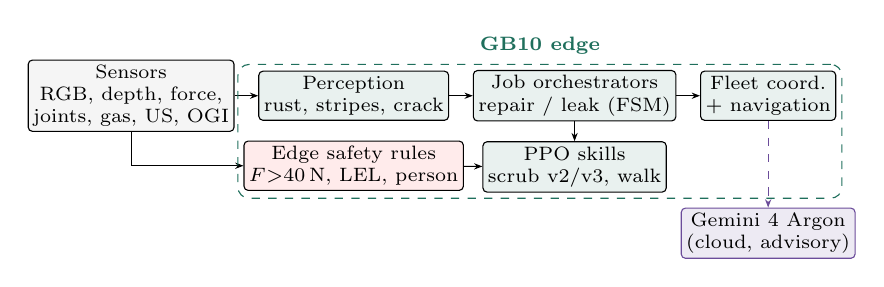
\begin{tikzpicture}[font=\scriptsize, node distance=2.5mm and 3mm,
  b/.style={draw, rounded corners=1.5pt, inner sep=1.8pt, align=center, fill=white},
  ar/.style={-{Stealth[length=3pt]}, thin}]
\node[b, fill=gray!8] (s) {Sensors\\RGB, depth, force,\\joints, gas, US, OGI};
\node[b, right=of s, fill=edge!10] (p) {Perception\\rust, stripes, crack};
\node[b, right=of p, fill=edge!10] (o) {Job orchestrators\\repair / leak (FSM)};
\node[b, below=of o, fill=edge!10] (pp) {PPO skills\\scrub v2/v3, walk};
\node[b, below=of p, fill=red!8] (safe) {Edge safety rules\\$F{>}40$\,N, LEL, person};
\node[b, right=of o, fill=edge!10] (f) {Fleet coord.\\+ navigation};
\node[b, below=11mm of f, fill=cloud!12, draw=cloud] (g) {Gemini 4 Argon\\(cloud, advisory)};
\draw[ar] (s) -- (p); \draw[ar] (p) -- (o); \draw[ar] (o) -- (pp); \draw[ar] (o) -- (f);
\draw[ar] (s.south) |- (safe.west); \draw[ar] (safe) -- (pp);
\draw[ar, dashed, cloud] (f) -- (g);
\node[draw=edge, dashed, rounded corners, fit=(p)(o)(pp)(safe)(f), inner sep=2pt,
  label={[edge,font=\scriptsize\bfseries]above:GB10 edge}] {};
\end{tikzpicture}
\end{center}

\hd{What's novel} {\scriptsize(one line each; \textcolor{note}{\textit{in progress}} = upgrade running, opt-in upgrades measured before/after in \fn{runs\_sample/novelty/})}\par
{\scriptsize\begin{itemize}[label=--]
\item \textbf{Scrub:} force is an RL action with a quadratic over-force cost: 76.8\% $\to$ 1.0\% episodes $>$40\,N; a CBF force shield (RLS stiffness) then takes calm $>$40\,N 0.8\% $\to$ 0\% and storm 11.5\% $\to$ 6.6\%.
\item \textbf{Storm:} storm-randomised fine-tune cuts the worst-case contact force 274\,N $\to$ 69\,N at full storm.
\item \textbf{Walking:} one gait for stowed \emph{and} deployed arm (payload $\alpha$ in obs): 1.94 falls/km (RMA adaptation \textcolor{note}{\textit{in progress}}).
\item \textbf{Pick-up:} Gemini Robotics-ER points at the grasp on unseen objects: on target 7\% $\to$ 97\%, 3-D error 26 $\to$ 0.5\,cm.
\item \textbf{Repair FSM:} soak-before-scrub and verify-before-paint with lens/gust/person safety states; 0 force violations with the sensor in the loop.
\item \textbf{Gas:} Bayesian particle filter + infotaxis finds the CH$_4$-only leak 64\% $\to$ 86\%, wrong-flange hand-offs 2 $\to$ 0.
\item \textbf{Fleet / Argon:} plans are rehearsed in a fast sim before use: bad-plan leak isolation 437 $\to$ 406\,s, 0 unsafe.
\item \textbf{Perception:} shift-gated test-time adaptation: storm-lens F1 0.47 $\to$ 0.95, clear-weather F1 0.993 unchanged.
\end{itemize}}

\hd{Honest caveats.} (i) The Isaac live repair run uses a \emph{colour stand-in} detector, not the LoRA model; the LoRA
F1 0.977 is published in \texttt{detection/RESULTS.md}, not re-measured here (the edge build of the sim-trained detector
scores 12/13 on held-out renders). (ii) Scrub legs are fixed in training (gravity off on the base); the trunk does not
sway except via the storm model. (iii) Walking and scrubbing are separate policies; some fleet demos move robots
kinematically. (iv) Gas results are a CPU mock with modelled sensor lags; the plume solver is validated against a
Gaussian plume (reported $\leq$4.5\% centreline error, 2--9\,m) but not against field data. (v) Gemini scrub numbers are
CPU-mock only (n=30); no Gemini action is ever executed without an edge rule and envelope check.
\end{multicols}
\end{document}
